\documentclass[11pt,letterpaper]{article}
\usepackage[T1]{fontenc}
\usepackage[utf8]{inputenc}
\usepackage{lmodern}
\pdfmapfile{+lm.map}
\pdfmapfile{+cm.map}
\pdfmapfile{+symbols.map}
\usepackage[margin=0.88in,headheight=15pt,headsep=18pt,footskip=26pt]{geometry}
\usepackage{amsmath,amssymb,amsthm,mathtools}
\usepackage{booktabs,tabularx,longtable,array}
\usepackage{graphicx,xcolor,microtype,enumitem,fancyhdr,titlesec,caption}
\usepackage[colorlinks=true,linkcolor=teal,citecolor=teal,urlcolor=teal,breaklinks=true]{hyperref}
\definecolor{teal}{HTML}{086F78}
\definecolor{navy}{HTML}{193248}
\definecolor{pale}{HTML}{EDF5F5}
\hypersetup{pdftitle={Ammons LLM Preamble},pdfauthor={Dean Ammons},pdfsubject={A semantics-aware probability framework for LLM response to domain content},pdfkeywords={language models, in-context learning, domain adaptation, influence, semantic equivalence, sparse domains}}
\titleformat{\section}{\large\bfseries\color{navy}}{\thesection}{0.65em}{}
\titleformat{\subsection}{\normalsize\bfseries\color{teal}}{\thesubsection}{0.6em}{}
\titlespacing*{\section}{0pt}{16pt}{7pt}
\titlespacing*{\subsection}{0pt}{11pt}{5pt}
\setlength{\parindent}{0pt}
\setlength{\parskip}{5.5pt plus 1pt minus 1pt}
\setlength{\emergencystretch}{2em}
\setlist{nosep,leftmargin=1.5em,topsep=5pt}
\captionsetup{font=small,labelfont=bf,skip=7pt}
\pagestyle{fancy}\fancyhf{}
\fancyhead[L]{\small\color{teal}AMMONS LLM PREAMBLE}
\fancyhead[R]{\small\color{navy}Dean Ammons}
\fancyfoot[C]{\small\thepage}
\renewcommand{\headrulewidth}{0.3pt}
\newtheorem{theorem}{Theorem}
\newtheorem{proposition}[theorem]{Proposition}
\newtheorem{corollary}[theorem]{Corollary}
\theoremstyle{definition}\newtheorem{definition}[theorem]{Definition}
\newcommand{\TV}{d_{\mathrm{TV}}}
\newcommand{\AIP}{\operatorname{AIP}}
\newcommand{\E}{\mathbb{E}}
\newcommand{\Prob}{\mathbb{P}}
\newcommand{\ind}{\mathbf{1}}
\newcommand{\R}{\mathbb{R}}
\newcommand{\calE}{\mathcal{E}}
\newcolumntype{Y}{>{\raggedright\arraybackslash}X}
\newcommand{\PilotPairs}{12}
\newcommand{\PilotContexts}{24}
\newcommand{\PilotAnswersPerArm}{24}
\newcommand{\PilotTreatmentCorrect}{24}
\newcommand{\PilotControlCorrect}{0}

\begin{document}
\thispagestyle{empty}
\begin{center}
{\small\sffamily\color{teal}RESEARCH PREPRINT\quad |\quad 12 NOVEMBER 2026}\par
\vspace{14pt}
{\LARGE\bfseries\color{navy}Ammons LLM Preamble}\par
\vspace{9pt}
{\large Dean Ammons}\par
\vspace{7pt}
{\normalsize A probability framework for behavioral influence through domain content}
\end{center}
\vspace{5pt}
\begin{abstract}
An interaction with specialized content can change a language model's behavior without establishing any historical source relationship. This paper defines influence operationally as a change in a model's distribution over role- and domain-preserving semantic outcomes under a specified content intervention. The Ammons Influence Probability is the probability, over a declared query population, that this distributional change exceeds a chosen threshold. Its companion mean effect has an exact minimum-disagreement coupling interpretation. Under an explicit evidence-pooling model, the pointwise effect factors as incorporated evidence divided by total effective information, multiplied by semantic discrepancy. We prove a conditional scarcity theorem, an exact dose threshold, invariance and coarsening properties, robustness bounds, and a finite-sample measurement bound. A local training derivation connects the same weighting principle to curvature and gradient alignment. An anonymous 25-entry, 19-group mathematical comparison corpus supplies measurement controls and dependence-aware balancing; it supplies no LLM exposure-response frequencies. Exact rational computation verifies the stated model identities. A separate pilot uses \PilotContexts{} fresh LLM contexts across \PilotPairs{} paired, newly generated microdomains: work exposure yields \PilotTreatmentCorrect{}/\PilotAnswersPerArm{} correct answers and matched control content yields \PilotControlCorrect{}/\PilotAnswersPerArm{}. This is an encounter-time result, not an estimate of hidden training support or a universal scarcity law. The contribution is a testable measurement framework with explicit assumptions and reproducible boundaries.
\end{abstract}
\vspace{3pt}
\noindent\textbf{Keywords:} language models; domain content; in-context learning; semantic equivalence; influence probability; effective evidence; sparse support.
\vspace{6pt}
\begin{center}\color{teal}\rule{0.96\linewidth}{0.6pt}\end{center}
\textbf{Central result.} For a semantic response law $P_r$, matched control $P_{0,r}$, query $q\sim Q_D$, and threshold $0<\epsilon<1$,
\begin{equation*}
\AIP_{r,\epsilon}=\Prob_{q\sim Q_D}\!\left\{\TV(P_r,P_{0,r})>\epsilon\right\}.
\end{equation*}
Under the declared pooling model, the quantity inside the threshold is exactly
\begin{equation*}
\widetilde\tau_r(q)=\frac{m_r(q)}{\kappa_D(q)+m_r(q)}\,\nu_W(q).
\end{equation*}
Here $m_r$ is incorporated evidence, $\kappa_D$ is effective background information mass, and $\nu_W$ is the work's semantic discrepancy from the control. These are distinct quantities. Their empirical values must be measured or calibrated; the equation does not infer them from the existence of matching source material.

\newpage
\section{Question, scope, and contribution}
The question is whether, and by how much, interaction with a domain-specific work changes an LLM's behavior on independently specified domain queries. A work may be a mathematical specification, a scientific argument, a technical manual, a program, or a set of demonstrations. The endpoint is an observable response distribution. Historical source attribution is outside the study.

Two regimes require separate controls. In the \emph{encounter regime}, the model receives the work in its current input while the evaluated parameter state is held fixed. In the \emph{training regime}, a specified learning procedure incorporates the work and the updated model is evaluated in a fresh context. Both can be measured with the same semantic response metric, but a context-only experiment does not establish a parameter update or persistence after context removal.

The phrase \emph{exotic content} is used here operationally rather than aesthetically. A work is relevant to the hypothesis when the evaluated system has weak support for its domain-specific consequences, the work differs semantically from the baseline response, and the system can take up some of that content. Unusual words, high surprise, or unfamiliar notation alone do not establish those conditions. A model may have little domain information yet fail to interpret the work; another may have substantial background knowledge and use that knowledge to interpret a new specification effectively.

The contribution has four parts. First, we define a probability with an explicit random unit and a semantic, rather than lexical, outcome space. Second, we derive a transparent support-and-exposure law inside an explicit mathematical model and give conditions under which it can fail as an LLM approximation. Third, we convert an anonymous mathematical comparison study into a balanced measurement-development panel without treating its source counts as behavioral samples. Fourth, we execute exact mathematical checks and a separate controlled LLM pilot. The framework synthesizes established probability and learning ideas; it does not claim the first observation of in-context adaptation or the invention of total variation.

\section{Related work and the unresolved measurement problem}
Few-shot language-model experiments show that instructions and demonstrations can change task performance without task-specific gradient updates \cite{brown2020}. Additional domain-adaptive and task-adaptive pretraining also changes performance in the studied domains \cite{gururangan2020}. These results support treating encounter and training exposure as distinct, experimentally meaningful regimes.

Bayesian interpretations explain some in-context behavior under explicit generative assumptions. Xie et al. analyze a mixture-of-hidden-Markov-models setting with shared latent concepts \cite{xie2022}; that theorem is not an unrestricted statement about concepts outside the modeled support. Controlled function-learning studies examine held-out functions within selected families \cite{garg2022}. Linear-model constructions and experiments connect in-context computation to learning algorithms and gradient-like updates \cite{akyurek2023,vonoswald2023}. They motivate a tractable surrogate but do not imply that every transformer implements the same scalar update.

Distributional properties matter. Chan et al. study rare classes, burstiness, and changing interpretations in constructed training distributions \cite{chan2022}. Kandpal et al. relate factual performance to relevant pretraining support and examine retrieval and retraining interventions \cite{kandpal2023}. These findings support controlled tests of support density. They do not supply a universal coefficient converting domain rarity into influence. In particular, training frequency, observable baseline accuracy, and effective information mass are different measurements.

Demonstration format and label-space information can account for improvements in some settings \cite{min2022}; prompt order and label biases also affect outcomes \cite{zhao2021}. Pan et al. distinguish recognition of a previously learned task from learning a new input-label mapping in context \cite{pan2023}. Consequently, a valid instrument should test work-specific operational consequences, preserve invalid outcomes, and include matched controls. The pilot below tests a newly specified function instance through direct and compositional queries. Its arithmetic building blocks remain familiar.

\section{A semantic definition of influence}
\subsection{The experimental contract}
Fix a protocol $\calE$ containing model identity, model state, exposure route, control content, decoding policy, tool access, reset conditions, query distribution, semantic evaluator, and observation horizon. Let $r\in\{c,t\}$ denote encounter or training exposure. Let $q\sim Q_D$ be a query from the declared domain population. The choice of $Q_D$ is substantive: weighting queries by deployment frequency answers a different question from weighting mathematical families equally.

For each query, a prespecified evaluator
\begin{equation}
\phi_q:\mathcal Y\longrightarrow\mathcal S_q
\label{eq:phi}
\end{equation}
maps raw responses to a finite or countable semantic outcome set. It binds input roles, output roles, admissible domain, state changes, precision, and relevant termination behavior. Only then does it discard incidental variable names or surface wording. Invalid, unclassifiable, and absent outputs receive explicit categories. General program equivalence is not assumed decidable: exact normalization may be restricted to a supported fragment, with other cases retained as unclassified.

Write the two response laws as
\begin{align}
P_{0,r}(s\mid q)&=\Prob\{\phi_q(Y_{0,r})=s\mid q,\calE\},\\
P_r(s\mid q,W)&=\Prob\{\phi_q(Y_r)=s\mid q,W,\calE\}.
\end{align}
The context control uses the same evaluated model state and matched irrelevant content where input length or format could matter. A work-specific training comparison uses matched initialization, optimization budget, and control training material; its evaluation excludes the target work from the inference context.

\begin{definition}[Pointwise effect and Ammons Influence Probability]
The semantic distribution change is
\begin{equation}
\tau_r(q;W)=\TV\!\left(P_r(\cdot\mid q,W),P_{0,r}(\cdot\mid q)\right)
=\frac12\sum_{s\in\mathcal S_q}|P_r(s\mid q,W)-P_{0,r}(s\mid q)|.
\label{eq:tau}
\end{equation}
Its average magnitude and threshold probability are
\begin{equation}
I_r(W;D)=\E_{q\sim Q_D}\tau_r(q;W).\label{eq:mean}
\end{equation}
\begin{equation}
\boxed{\AIP_{r,\epsilon}(W;D,\calE)
=\Prob_{q\sim Q_D}\{\tau_r(q;W)>\epsilon\}.}\label{eq:aip}
\end{equation}
\end{definition}

The random unit in Equation~\eqref{eq:aip} is a domain query drawn under the declared protocol. AIP is the probability that its effect exceeds a chosen materiality threshold. It is not the probability that a particular previously observed answer had an unobserved origin. The full threshold curve is more informative than an unexplained single cutoff.
Equations~\eqref{eq:mean}--\eqref{eq:aip} condition on a fixed work. A study that samples work instances uses the joint version, replacing $q\sim Q_D$ with $(W,q)\sim Q_D$ and averaging the same pointwise effect. All proofs below continue to apply to that declared joint population. The pilot uses this joint version; it does not estimate the effect of one fixed external work.

\begin{proposition}[Bounds and threshold integration]
$0\le \tau_r,I_r,\AIP_{r,\epsilon}\le1$, and $I_r=0$ exactly when $P_r=P_{0,r}$ for $Q_D$-almost every query. Furthermore,
\begin{equation}
I_r=\int_0^1\AIP_{r,\epsilon}\,d\epsilon.
\label{eq:layercake}
\end{equation}
For $0<\epsilon<1$,
\begin{equation}
\max\!\left(0,\frac{I_r-\epsilon}{1-\epsilon}\right)
\le\AIP_{r,\epsilon}
\le\min\!\left(1,\frac{I_r}{\epsilon}\right).
\label{eq:meanbounds}
\end{equation}
\end{proposition}
\begin{proof}
Total variation is in $[0,1]$ and vanishes exactly for equal measures. A nonnegative random variable has mean zero exactly when it is zero almost surely. For $x\in[0,1]$, $x=\int_0^1\ind\{x>u\}\,du$; taking expectations proves Equation~\eqref{eq:layercake}. If $p=\Prob(\tau>\epsilon)$, then $\epsilon p\le\E\tau\le\epsilon(1-p)+p$. Rearranging gives Equation~\eqref{eq:meanbounds}.
\end{proof}

\subsection{Why this metric has a probability interpretation}
\begin{theorem}[Minimum semantic disagreement]
For any fixed query and all couplings $\Gamma(P_0,P_r)$ of the two semantic response laws,
\begin{equation}
\tau_r(q)=\min_{\gamma\in\Gamma(P_0,P_r)}\Prob_\gamma(S_r\ne S_0).
\label{eq:coupling}
\end{equation}
\end{theorem}
\begin{proof}
A coupling can put at most $\min\{P_0(s),P_r(s)\}$ on the diagonal cell $(s,s)$. Thus its agreement probability is at most $\sum_s\min\{P_0(s),P_r(s)\}=1-\tau_r$. Put exactly this common mass on the diagonal. The remaining masses have disjoint supports and can be coupled arbitrarily; every remaining outcome disagrees. This achieves disagreement $\tau_r$.
\end{proof}
This is the standard coupling characterization of total variation \cite{levin2017}, specialized to semantic outcomes. It gives the smallest disagreement rate compatible with the two laws. Two independent model draws need not realize that coupling: they can disagree even when the laws are identical. A changed single answer is therefore not, by itself, an estimate of Equation~\eqref{eq:tau}.

\begin{proposition}[Names, coarsening, and aligned gain]
A bijective relabeling of semantic outcomes leaves $\tau_r$ unchanged. For a deterministic coarsening $T$,
\begin{equation}
\TV(T_\#P_r,T_\#P_0)\le\TV(P_r,P_0).
\label{eq:coarsen}
\end{equation}
For any prespecified score $u_q(s)\in[0,1]$ measuring agreement with held-out consequences of the work, define
\begin{equation}
G_r=\E_q\sum_s u_q(s)\{P_r(s\mid q,W)-P_{0,r}(s\mid q)\}.
\label{eq:gain}
\end{equation}
Then $|G_r|\le I_r$.
\end{proposition}
\begin{proof}
A bijection permutes the absolute differences in Equation~\eqref{eq:tau}. A coarse-cell difference is a sum of fine-cell differences, so the triangle inequality proves Equation~\eqref{eq:coarsen}. For a signed difference of two probability laws, the total positive mass equals TV. A function in $[0,1]$ can collect at most that mass and at least its negative. Apply the resulting bound pointwise and average.
\end{proof}
This separates influence from favorable adoption. Rejection, distraction, or error can produce a distribution change with zero or negative aligned gain. A useful report includes both the general change and its direction under the stated task score.
The relabeling result concerns the measurement's semantic labels. It does not assert that an LLM responds identically to every renamed or paraphrased prompt; that behavioral invariance is a separate empirical control.

\section{The support-and-exposure equation}
\subsection{Three quantities that must remain separate}
Let $R_W(\cdot\mid q)$ be a declared reference law for the work's implications. It can be deterministic when a specification has an exact answer. It need not represent external truth; it specifies the content whose uptake is being measured. Define
\begin{equation}
\nu_W(q)=\TV(R_W(\cdot\mid q),P_{0,r}(\cdot\mid q)).
\label{eq:nu}
\end{equation}
Let $\kappa_D(q)>0$ denote effective background information mass in declared evidence units, and let $m_r(W,q)\ge0$ denote evidence effectively incorporated through route $r$. Neither is automatically a number of tokens, documents, gradient steps, or retrieved files. Exposure can be present while $m_r=0$, and repeated text need not add independent information.

\begin{table}[htbp]\centering\small
\begin{tabularx}{\linewidth}{p{0.13\linewidth}YY}
\toprule
Quantity & Meaning & What does not identify it by itself\\\midrule
$\kappa_D$ & Strength of relevant background information & Unusual vocabulary; a single low baseline accuracy; raw corpus size\\
$m_r$ & Work evidence incorporated for this probe & Merely placing text in a prompt; repeated token count\\
$\nu_W$ & Semantic departure of the work from the control law & Source age; identical spelling; an asserted novelty label\\
$\rho_r$ & Error of the proposed pooling approximation & A successful fit on the same data used to choose parameters\\
\bottomrule
\end{tabularx}
\caption{The model parameters have distinct operational roles. Estimation needs intervention data and declared units.}
\label{tab:parameters}
\end{table}

The proposed pooling model is
\begin{equation}
\widetilde P_r(\cdot\mid q,W)
=\frac{\kappa_D(q)P_{0,r}(\cdot\mid q)+m_r(W,q)R_W(\cdot\mid q)}{\kappa_D(q)+m_r(W,q)}.
\label{eq:pool}
\end{equation}
It is a falsifiable response model, not an identity satisfied by every LLM. It restricts an exposed response vector to the line segment joining the control law and the work-reference law.

\subsection{An exact derivation and conditional theorem}
For a finite outcome set with $P_0(s)>0$, assign a categorical probability vector the Dirichlet prior $\alpha_s=\kappa_D P_0(s)$. A weighted evidence likelihood proportional to $\prod_s p_s^{c_s}$, with $c_s=m_rR_W(s)\ge0$, gives posterior parameters $\alpha_s+c_s$. Its predictive mean is exactly Equation~\eqref{eq:pool}. Fractional counts are a declared weighted-likelihood model. Exact zero probabilities require an explicit support model or a positive-smoothing limit; a zero empirical frequency is not proof of zero support.

\begin{theorem}[Exact factorization and conditional scarcity]
Under Equation~\eqref{eq:pool},
\begin{equation}
\boxed{\widetilde\tau_r(q;W)
=\frac{m_r(W,q)}{\kappa_D(q)+m_r(W,q)}\,\nu_W(q).}
\label{eq:factor}
\end{equation}
Consequently,
\begin{equation}
\boxed{\widetilde{\AIP}_{r,\epsilon}
=\Prob_{q\sim Q_D}\left\{
\frac{m_r(W,q)\nu_W(q)}{\kappa_D(q)+m_r(W,q)}>\epsilon\right\}.}
\label{eq:modelaip}
\end{equation}
Holding the other quantities fixed, for $m>0$ and $\nu>0$,
\begin{equation}
\frac{\partial\widetilde\tau}{\partial\kappa}
=-\frac{m\nu}{(\kappa+m)^2}<0,
\qquad
\frac{\partial\widetilde\tau}{\partial m}
=\frac{\kappa\nu}{(\kappa+m)^2}>0.
\label{eq:derivatives}
\end{equation}
For $0<\epsilon<\nu$, a material effect occurs exactly when
\begin{equation}
\boxed{m>\frac{\epsilon\kappa}{\nu-\epsilon}.}
\label{eq:threshold}
\end{equation}
\end{theorem}
\begin{proof}
Subtract $P_0$ from Equation~\eqref{eq:pool}. The result is $\lambda(R_W-P_0)$ where $\lambda=m/(\kappa+m)\ge0$. Homogeneity of the absolute-value sum gives Equation~\eqref{eq:factor}; substituting it into Definition~1 gives Equation~\eqref{eq:modelaip}. Differentiation gives Equation~\eqref{eq:derivatives}. Finally $m\nu/(\kappa+m)>\epsilon$ is equivalent to $m(\nu-\epsilon)>\epsilon\kappa$, and division is valid when $\nu>\epsilon$.
\end{proof}

This is the precise scarcity claim: \emph{for the same incorporated evidence and semantic discrepancy, weaker relevant background support produces a larger incremental response shift within the declared model}. If $m=0$ or $\nu=0$, the shift is zero. If $\nu\le\epsilon$, no finite dose crosses the strict threshold. As $m\to\infty$, the shift saturates at $\nu$, not necessarily one. For $m>0$, the limit $\kappa\downarrow0$ also gives $\nu$; the simultaneous zero-mass case is not a proper prior.

For illustration only, take $m=2$ and $\nu=0.8$. Background masses $\kappa=0.2,2,20$ give shifts $0.7273,0.4000,0.0727$, respectively. These are specified-model calculations, not fitted estimates from the anonymous corpus or the LLM pilot. Figure~\ref{fig:pool} displays the dose and support relationship.

\begin{figure}[htbp]\centering
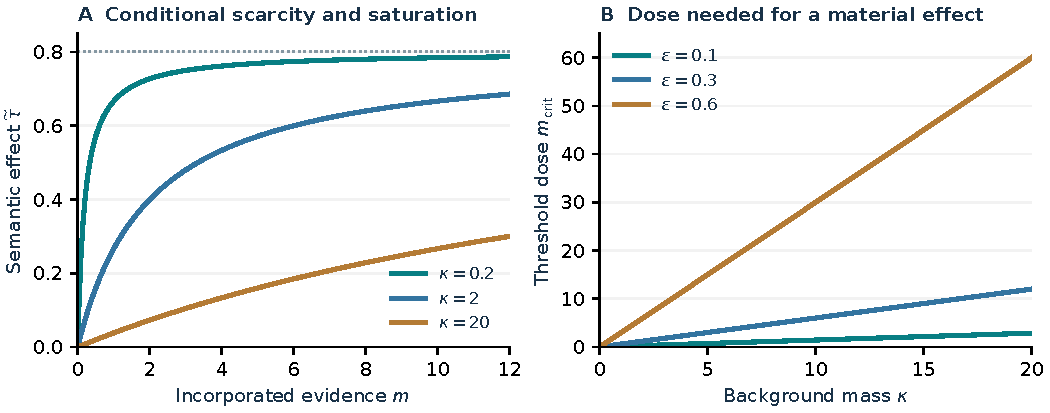
\includegraphics[width=\linewidth]{figures/pooling.pdf}
\caption{Specified-model illustration, not an empirical fit. Left: effect versus effective incorporated evidence for three background masses at fixed $\nu=0.8$. Right: the exact dose needed to exceed a materiality threshold when $\nu=0.8$. Effects and thresholds are consequences of the declared pooling law.}
\label{fig:pool}
\end{figure}

\subsection{Why sparsity does not force uptake}
There are two different notions of rarity. Small $\kappa$ means weak relevant information mass. A small prior probability $\pi_0$ for a particular claim means the model strongly or weakly disfavors that claim; its concentration is not determined by $\pi_0$. Under a fixed finite Bayes factor $B$,
\begin{equation}
\pi_1=\frac{\pi_0B}{1-\pi_0+\pi_0B},
\qquad \lim_{\pi_0\downarrow0}\pi_1=0.
\label{eq:bayesfactor}
\end{equation}
Thus increasingly surprising content need not increasingly dominate. The statement that an arbitrary model \emph{must} change when content is exotic is false: a model that ignores the supplied work has $m=0$ and equal response laws, regardless of the work's rarity. This counterexample specifies exactly why uptake is an independent factor.

Domain training can change all three factors. It may increase $\kappa$, improve interpretation and therefore $m$, and move the control response, changing $\nu$. The sign of the total effect is then not fixed by the partial derivative in Equation~\eqref{eq:derivatives}. A study must either control these other factors or measure them instead of interpreting an unconditional rarity correlation as the theorem.

\subsection{Misspecification and parameter identification}
Define the discrepancy between an actual exposed law and the surrogate as
\begin{equation}
\rho_r(q)=\TV(P_r(\cdot\mid q,W),\widetilde P_r(\cdot\mid q,W)).
\end{equation}
The reverse triangle inequality yields
\begin{equation}
|\tau_r(q)-\widetilde\tau_r(q)|\le\rho_r(q),
\qquad |I_r-\E_q\widetilde\tau_r(q)|\le\E_q\rho_r(q),
\label{eq:robust}
\end{equation}
and therefore
\begin{equation}
\Prob_q\{\widetilde\tau_r-\rho_r>\epsilon\}
\le\AIP_{r,\epsilon}
\le\Prob_q\{\widetilde\tau_r+\rho_r>\epsilon\}.
\label{eq:aiprobust}
\end{equation}
These bounds follow by event inclusion and keep approximation error visible. A response vector outside the control-to-reference line segment falsifies the scalar pooling law even when the work-aligned score increases.

If $P_0\ne R_W$ and the model is correct, a fitted mixture coefficient identifies $m/\kappa=\lambda/(1-\lambda)$, subject to the endpoint cases. It does not identify $m$ and $\kappa$ separately: scaling both by the same positive constant preserves every prediction. An externally defined dose scale or independent support measurement is needed. For a dose model $m=ad$, the identifiable ratio may be $\kappa/a$, not an actual number of training documents. Repetition, exposure length, and independent semantic information should remain separately recorded.

\section{The training regime}
The behavioral definitions do not depend on how an intervention is implemented. A useful local derivation nonetheless shows why background strength and alignment enter a training effect. Let the control objective $L_0$ have a stationary point $\theta_0$, and consider $L_0(\theta)+aL_W(\theta)$. Define $H_0=\nabla^2L_0(\theta_0)$, $H_W=\nabla^2L_W(\theta_0)$, and $g_W=\nabla L_W(\theta_0)$. A quadratic expansion gives
\begin{equation}
\delta\theta\simeq-a(H_0+aH_W)^{-1}g_W.
\label{eq:training}
\end{equation}
For a differentiable semantic-score probability $f_q(\theta)$,
\begin{equation}
f_q(\theta_0+\delta\theta)-f_q(\theta_0)
\simeq-a\nabla f_q(\theta_0)^\mathsf T(H_0+aH_W)^{-1}g_W.
\label{eq:alignment}
\end{equation}
Equations~\eqref{eq:training}--\eqref{eq:alignment} assume $H_0+aH_W$ is invertible and describe a local stationary displacement; positive definiteness is sufficient for the quadratic stationary point to be a minimum. These expressions follow by linearizing the stationarity equation and then the response function. If $H_0$ is positive definite and the derivatives are sufficiently regular, the implicit function theorem gives
\begin{equation}
\delta\theta=-aH_0^{-1}g_W+O(a^2).
\end{equation}
The local quadratic formula is exact for quadratic objectives; it is an approximation otherwise. Actual neural losses may have singular or indefinite Hessians, so a declared regularized subspace or stronger local assumptions are required.

Weak curvature amplifies only directions reached by the update and observed by the probe. Orthogonal gradients, saturation, or cancellation can produce no aligned effect. Thus sparse support cannot be inferred solely from the existence of a large parameter change, and a large parameter change need not produce a large semantic response change.

A one-dimensional quadratic case gives a direct bridge. Let
\begin{equation}
L_0(z)=\tfrac12\kappa(z-z_0)^2,
\qquad aL_W(z)=\tfrac12m(z-z_W)^2.
\end{equation}
The unique minimizer for $\kappa>0,m\ge0$ is
\begin{equation}
z_* =\frac{\kappa z_0+mz_W}{\kappa+m}.
\label{eq:quadratic}
\end{equation}
Differentiating the summed objective proves this equation. It recovers the pooling weight in an exact training model; it does not show that a full LLM has a one-dimensional quadratic loss.

A complete training experiment should randomize background domain support and work-specific training separately, use matched compute, and evaluate updated checkpoints with the work absent from the test context. The present paper derives this regime and grounds it in prior training studies; it does not report a new LLM weight-update experiment.

\section{Balancing the anonymous measurement corpus}
\subsection{What the antecedent observations contribute}
The antecedent corpus is a privately held mathematical source-comparison study, anonymized here by withholding owner identities, source links, exact dates, original formulae, source-level names, and program bindings. Its aggregates are observations about the measurement instrument. They are not labeled LLM exposures. The complete aggregate-to-design mapping appears in Appendix~\ref{app:panel}; no source equation is reproduced.

The reviewed set contains 25 component entries in 19 dependence groups: one group has three entries, four groups have two entries each, and fourteen groups are singletons. Two nonconstant components in one group have native execution confirmation under an explicitly shared mathematical interpretation. Their original type declarations also preserve a domain mismatch. That combination is valuable: it validates a restricted positive case while preventing a type-erasing universal match.

The broad candidate population contains hundreds of conditional scalar forms represented by many thousands of source-pair records, together with notation candidates and a separately reviewed relation. That relation is already included in the 25-entry set. Intersections between the broad and reviewed populations are not fully resolved, so their counts cannot be added as disjoint observations. The compressed broad rows were not independently decoded in the antecedent investigation; their totals retain the status of saved aggregate results. Nonessential legacy inventory numbers are generalized here to reduce source-identifying cues; the dependence counts needed for the balancing equation are retained.

Source chronology contains witnesses in both temporal orderings and cases with incomplete original anchors. These classifications inform record completeness only. They do not enter a prior probability, a behavioral response denominator, or an influence likelihood. Integrity checks and source-order corrections likewise constrain the instrument without supplying exposed and unexposed model outputs.

\subsection{Exact dependence-aware weights}
Let group $g$ contain $n_g$ entries and let entry $j$ have $v_{gj}$ eligible variants. An equal-group development measure assigns
\begin{equation}
w_{gjk}=\frac{1}{19\,n_g\,v_{gj}},
\qquad
I_r^{\mathrm{bal}}
=\frac1{19}\sum_{g=1}^{19}\E_{q\sim Q_g}\tau_r(q).
\label{eq:balance}
\end{equation}
With one score per entry, row weights are $1/57$ in the three-entry group, $1/38$ in each two-entry group, and $1/19$ in each singleton. They sum to one and every group contributes exactly $1/19$. Additional source locations remain provenance rather than statistical replication. This weighting defines an equal-family target population; it is not automatically the correct deployment distribution.

The instrument must preserve five controls: role-preserving renaming, domain and type restrictions, all eligible retrieval candidates, exact source localization, and composition or state effects. The antecedent findings include failures in each relevant area. The native positive subset and exact-arithmetic suites therefore guide the evaluator's inclusion rules and negative controls. They are not converted into thousands of independent behavioral samples.

\begin{proposition}[Source-only observations do not identify AIP]
Let $O$ contain only mathematical source matches, chronology, source identity checks, and execution comparisons of source fragments. Assume the scorer admits at least two attainable semantic outcomes for $Q_D$-almost every query. If $O$ contains no LLM intervention-response laws, it does not identify $\AIP_{r,\epsilon}$ for $0<\epsilon<1$.
\end{proposition}
\begin{proof}
Hold all components of $O$ fixed. One response model can satisfy $P_r=P_0$ for every query, giving AIP zero. Another can assign disjoint deterministic semantic outcomes to control and exposure for every query, giving AIP one for every $\epsilon<1$. Neither construction changes $O$. The same observed $O$ therefore permits different AIP values.
\end{proof}
This establishes the precise role of the earlier findings: they balance and challenge the semantic instrument. New exposure-response observations are needed to calibrate a behavioral probability.

\section{Estimation, uncertainty, and falsification}
\subsection{Finite semantic distributions}
For a fixed query with $K$ prespecified categories, collect $n_0,n_r$ independent outputs under the two conditions. Define empirical response laws and $\widehat\tau=\TV(\widehat P_r,\widehat P_0)$. Let
\begin{equation}
u_a=\sqrt{\frac{\log(4K/\alpha)}{2n_a}},\quad a\in\{0,r\},
\qquad b=\min\!\left\{1,\frac K2(u_0+u_r)\right\}.
\end{equation}
Then
\begin{equation}
\Prob\{|\widehat\tau-\tau|\le b\}\ge1-\alpha.
\label{eq:tvci}
\end{equation}
\begin{proof}
For each category frequency, the two-sided bounded-sum inequality gives a failure probability at most $2e^{-2n_au_a^2}=\alpha/(2K)$ \cite{hoeffding1963}. A union bound over both arms and all $K$ categories gives simultaneous cell accuracy. The reverse triangle inequality bounds the TV error by one half of the sum of the two $\ell_1$ frequency errors, at most $K(u_0+u_r)/2$.
\end{proof}
The bound is conservative and may be uninformative for small samples or a large ontology. That is a property of the data requirement, not a reason to replace the interval with a precise-looking unsupported point estimate. A binary prespecified consequence can use a sharper Bernoulli calculation, but such coarsening measures only that consequence.

For independently sampled queries $q_1,\ldots,q_J$, obtain simultaneous pointwise intervals $[\ell_j,u_j]$ at total failure probability $\alpha/2$. Set $\widehat L=J^{-1}\sum_j\ind\{\ell_j>\epsilon\}$ and $\widehat U=J^{-1}\sum_j\ind\{u_j>\epsilon\}$. With $h=\sqrt{\log(4/\alpha)/(2J)}$,
\begin{equation}
\left[\max(0,\widehat L-h),\min(1,\widehat U+h)\right]
\label{eq:aipci}
\end{equation}
is a coverage-$1-\alpha$ interval for AIP. On the simultaneous-interval event, the true sample threshold frequency lies between $\widehat L$ and $\widehat U$; a bounded-sum inequality controls its deviation from the population threshold probability. The two error allowances sum to $\alpha$.

Queries sharing a conversation, training run, work, or generation seed can be dependent. The independent unit must be the corresponding cluster, or the uncertainty calculation must model that dependence. Repeated answers inside one context do not become independent exposure trials.

\subsection{A bound available from aligned transfer alone}
Fix a benchmark of $N$ domain pairs. Assume their response pairs are independent conditional on that benchmark and the stable protocol. Let scores $S_{i,r},S_{i,0}\in[0,1]$ give differences $D_i=S_{i,r}-S_{i,0}\in[-1,1]$. Then $\widehat G=N^{-1}\sum_iD_i$ estimates $G=N^{-1}\sum_i\E D_i$, the aligned gain under uniform benchmark weighting. Identical response distributions across domains are not required. A one-sided bound is
\begin{equation}
G_r\ge \widehat G-\sqrt{\frac{2\log(1/\alpha)}{N}}
\quad\text{with probability at least }1-\alpha.
\label{eq:gainci}
\end{equation}
The proof applies the bounded-sum inequality to independent variables of range two. Since $I_r\ge G_r$, the positive part of this lower bound also bounds the mean semantic effect. Equation~\eqref{eq:meanbounds} then gives a conservative lower bound on AIP for the same finite benchmark. This does not recover the pointwise TV values, the complete threshold curve, or an unseen-domain population effect. Extending it to a generator population requires an appropriate sampling argument in addition to response independence.

\subsection{Individual induced responses and missing measurements}
For binary potential outcomes $A_0,A_r$, marginal rates $p_0,p_r$ imply the sharp bounds
\begin{equation}
\max(0,p_r-p_0)\le\Prob(A_r=1,A_0=0)\le\min(p_r,1-p_0).
\label{eq:pns}
\end{equation}
To prove them, write the middle quantity as $p_r-\Prob(A_r=1,A_0=1)$ and apply the intersection bounds. Individual monotonicity would collapse the interval to $p_r-p_0$, but positive mean gain does not establish monotonicity. This distinction is consistent with standard probability-of-causation identification results \cite{tianpearl2000}; the primary AIP estimand avoids requiring this unobserved coupling.

For fixed weights $w_i$ summing to one, let only set $O$ have measured effects with intervals $[L_i,U_i]$. The complete target mean obeys
\begin{equation}
\sum_{i\in O}w_iL_i\le I_r\le
\sum_{i\in O}w_iU_i+\sum_{i\notin O}w_i.
\label{eq:missing}
\end{equation}
Every unmeasured effect lies in $[0,1]$, proving the bound. Renormalizing observed cases instead defines a different, measured-only population. Inaccessible source rows and unresolved labels must not silently become zero effects.

\subsection{How the model can fail}
The pooling law is rejected for a probe if its exposed distribution lies outside the permitted line segment beyond measurement error. Its scalar parameterization is inadequate when different semantic outcomes require incompatible mixing weights. The scarcity claim is not tested by changing background support while also changing interpretability, dose, or work discrepancy without accounting for those changes. A successful model fit on one set of domain families should be evaluated on held-out families, with calibration errors and interval coverage reported. A work that produces no measured shift is a valid null result.

\section{Validation results}
\subsection{Exact rational verification of the model}
The supplied standard-library program enumerates all 15 three-category probability vectors on a quarter grid, all baseline/reference pairs, background masses $\{1,2,4\}$, and evidence masses $\{0,1,3,8\}$. It verifies the identities with rational arithmetic, avoiding floating-point tolerance as a substitute for equality.
\begin{table}[htbp]\centering\small
\begin{tabularx}{\linewidth}{YrY}
\toprule
Property & Cases & Result and interpretation\\\midrule
Exact pooling factorization & 2,700 & All exact; checks Equation~\eqref{eq:factor} on the stated grid\\
Applicable strict-threshold equivalence & 3,024 & All exact; preserves the strict inequality and boundary conditions\\
Scarcity comparison under doubled background mass & 2,025 & All nonzero-dose cases satisfy the stated monotonicity\\
Residual triangle bound & 40,500 & All exact against every actual-response vector on the grid\\
Group weights and zero/threshold boundaries & Declared cases & Exact normalization and edge behavior\\
\bottomrule
\end{tabularx}
\caption{Numerical verification of stipulated mathematics. These are deterministic model checks, not LLM samples. The general claims are proved in the preceding sections.}
\label{tab:exact}
\end{table}
The calculations validate implementation of the equations and their boundaries. They do not empirically establish that an LLM follows the pooling approximation. The source program prints the counts and raises an error if an asserted property fails.

\subsection{A controlled encounter-time pilot}
The pilot used \PilotPairs{} newly generated microdomains, each evaluated in two fresh, history-free assistant contexts. Each context returned two outputs: a direct application and a nested composition on held-out inputs. Domain notes and queries were fixed before the first model call. Work/control order was randomized within pairs, and pair order was randomized. Planned prompts contained 733 characters; one dispatched prompt omitted a single formatting space, giving 732 characters without changing the rule or query. The actual prompt and this deviation were retained, and the invocation was not repeated. No answer key or opposite-arm response was available to an evaluated context; the prompts prohibited tool use.

The target was a newly named operation on the residues $\{0,\ldots,10\}$:
\begin{equation}
u\star v=(au+bv+c)\bmod11,
\label{eq:pilotrule}
\end{equation}
with independently generated coefficients subject to nonzero, unequal operand coefficients. This equation is a new experimental surrogate, not an equation from the anonymous comparison corpus. The exposure note defined the queried operation. The control note had the same form but defined a different named operation with independently sampled coefficients; both notes said rules were local to their names. Both conditions requested the same two target queries and integer-only JSON answers, with a best estimate if the target rule was unspecified.

The particular rule instances were newly generated and unavailable in the control note. This establishes a controlled information difference about those instances; it does not establish that modular arithmetic, affine functions, or their compositions were absent from pretraining. Correct direct answers show work-specific interpretation; correct nested answers additionally show execution on an unseen composition. No worked target answers were included.

The experiment used the session's fresh-subagent LLM interface with inherited model selection and no conversation-history fork. An exact model release, decoding temperature, sampling seed, and backend checkpoint were not exposed through that interface. The reported result therefore identifies the evaluated interface and protocol, not an independently frozen public checkpoint. All issued prompts, returned responses, invocation order, and deterministic scores are retained in the public reproduction materials; internal session identifiers are omitted.

\begin{table}[htbp]\centering
\begin{tabular}{lrr}\toprule
Outcome & Work exposure & Matched control\\\midrule
Direct interpretation & 12/12 & 0/12 \\
Nested composition & 12/12 & 0/12 \\
Total correct answers & 24/24 & 0/24 \\
Valid response objects & 12/12 & 12/12 \\
\bottomrule\end{tabular}
\caption{Observed pilot results. Answers within one context are clustered; the primary analysis has 12 domain pairs.}
\label{tab:pilot}
\end{table}
All 12 paired domain differences were +1 on the mean-correctness scale, so the observed paired mean gain was $\widehat G=1.0$. Every control response was $(5,5)$; none of the pre-generated answer keys was 5. The generated dataset was fixed before any response, with no dataset selection based on outcomes.

The predeclared paired-label test enumerated all $2^{12}=4096$ assignments. Its directional null-tail probability was $1/4096=0.000244140625$, and its two-sided probability was $2/4096=0.00048828125$. The exact sign test agreed. These results require the stated paired exchangeability and domain-level independence assumptions.

\begin{figure}[htbp]\centering
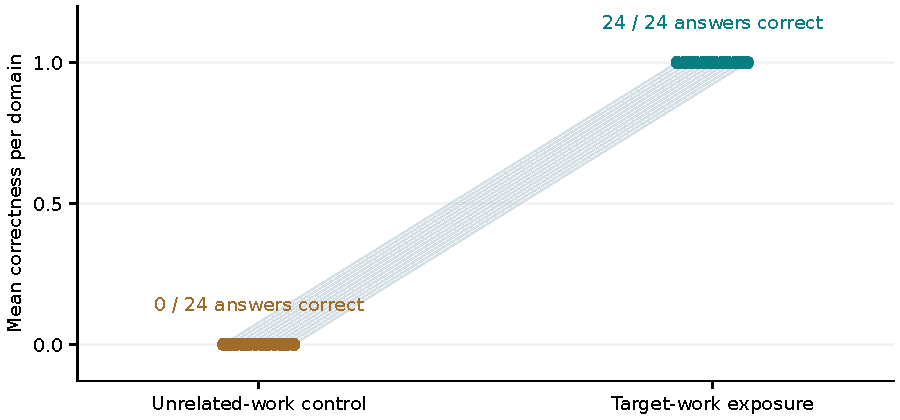
\includegraphics[width=0.85\linewidth]{figures/pilot.pdf}
\caption{Observed encounter-time pilot. Each mark is one domain-paired mean score, based on two answers in one fresh context per condition. There are 12 instances of one generated function class. No per-query output-distribution or training-support estimate is plotted.}
\label{fig:pilot}
\end{figure}
\textbf{Exploratory bound.} Separately from the predeclared tests, Equation~\eqref{eq:gainci} with $\alpha=0.05$ gives $G\ge 0.2934$ and hence $I\ge 0.2934$ for the same fixed 12-domain benchmark, conditional on independent response pairs and a stable interface. At an illustrative threshold $\epsilon=0.10$, Equation~\eqref{eq:meanbounds} gives $\AIP_{0.10}\ge 0.2149$ on that same coverage event. This is a conservative one-sided 95\% bound under those assumptions, not a point estimate or a coefficient fitted to the pooling law. The backend's independence and checkpoint stability were not directly observable.


The two answers inside one context were scored together. The analysis unit is the domain pair, not an individual answer or token. These are 12 instances of one function class, not 12 independent mathematical families. For the bound on $I_r$, the query population selects uniformly from the fixed 12-domain benchmark and then chooses its direct or nested probe with probability $1/2$. Names were generated uniquely across the protocol, so an IID distribution of complete named tasks is not assumed. The exact paired calculation flips the sign of each whole-domain score difference and enumerates all $2^{\PilotPairs}$ assignments under the paired exchangeability null. The reported $p$-value addresses this experimental comparison and is not a probability that the hypothesis is true.

Equation~\eqref{eq:gainci} supplies a conservative, assumption-dependent lower bound on mean effect for the same fixed benchmark, conditional on independent response pairs. Because the pilot has one response per arm at each query, it does not estimate a full multicategory law for each query, identify $\kappa_D$ or $m_r$, or fit the scarcity curve. It also does not show persistent learning or a training update. A repeat with a versioned model and controlled decoding is needed for broader reproducibility.

\section{A complete empirical calibration study}
The next calibration study should cross three independently specified factors: relevant background support, exposure content, and exposure dose. For actual training support, use controlled model training with known domain-example counts and matched compute. For a frozen black-box LLM, measure baseline coverage on separate probes and call that covariate \emph{observable baseline coverage}, not a recovered training frequency. Changing a background document in a prompt manipulates contextual support, not training support.

Within each support stratum, randomize correct work, coherent irrelevant work, and a changed-rule or meaning-destroyed control. Preserve format, length, ordering policy, and task difficulty as far as the intended intervention allows. Include role-preserving paraphrases and renamings. Evaluation should hold out inputs, compositions, and, where feasible, whole task families; it should not reward literal repetition of exposure examples.

Estimate response laws with repeated independent contexts. Fit a dose model and the pooling segment on one family partition, then evaluate probability calibration and the residual $\rho_r$ on held-out families. Report the full AIP threshold curve, mean effect, aligned gain, invalid-output rate, and between-family variation. Keep training-run seeds, context clusters, and domain families intact during uncertainty estimation. Predefine stopping rules and the primary threshold before inspecting results.

For the training arm, evaluate in a fresh context after the update; for the encounter arm, define a separate context-removal endpoint if persistence is of interest. If the interface provides no weight-update or memory control, the study should restrict its claim to the observable encounter condition. A trained-domain system and a sparsely supported system can both be influenced, but their relative effect is an empirical comparison after uptake and discrepancy are accounted for.

\section{Discussion}
The framework resolves an ambiguity in the phrase \emph{probability of influence}. The mean effect $I_r$ measures how much semantic probability mass changes; AIP measures how often a query's effect exceeds a threshold. The probability of an individually induced answer is a third quantity, with separate identification requirements. Reporting these quantities under their own names prevents a source-overlap count, an observed answer difference, and a behavioral probability from being treated as interchangeable.

The conditional scarcity result is useful because it is both positive and falsifiable. When a work is incorporated and semantically differs from the baseline, weaker background information increases the response shift in the pooling model. The equation also shows precisely when that conclusion fails: no uptake, no discrepancy, an insufficient dose, a support restriction, or a poor fit to the scalar model. Model competence can increase uptake while prior training increases resistance, so the total relation between familiarity and influence can be nonmonotonic.

The anonymous development corpus contributes unusually demanding semantic controls: equal effects under different representations, type-boundary failures, repeated manifestations of one family, and procedural comparisons whose complete contracts remain different. Those controls improve the meaning of a measured response shift. Their large deterministic check counts add no LLM sample size. Their chronology adds no behavioral likelihood. Public reproducibility of the withheld corpus is limited to its released aggregate description; the mathematical proofs and new pilot are separately inspectable.

The pilot establishes a bounded encounter-time result for newly specified function instances at the evaluated interface. It cannot distinguish every possible internal computation, estimate hidden pretraining frequency, or validate the pooling coefficients across scientific domains. Its purpose is to connect the formal endpoint to actual model outputs while keeping those broader hypotheses open to controlled measurement.

\section{Conclusion}
The Ammons Influence Probability is a domain-conditioned probability of a material semantic response change after a specified content intervention. Its companion mean effect has a minimum-disagreement interpretation, and the evidence-pooling model yields the exact relation $\widetilde\tau=m\nu/(\kappa+m)$. Under its stated conditions, sparse relevant background support amplifies fixed incorporated evidence. The mathematics supplies proofs, thresholds, null cases, and error bounds; the executed pilot supplies a separate observation of encounter-time uptake. Together they provide a reproducible starting point for measuring influence from specialized content while preserving the distinction between semantic measurement, model assumptions, and empirical calibration.

\clearpage
\appendix
\section{Complete anonymous balancing panel}\label{app:panel}
The table accounts for the retained findings at the level needed for measurement design. Units are preserved; none is counted as an LLM intervention trial. Source identities, dates, original equations, and original family labels are withheld.
\small
\begin{longtable}{p{0.34\linewidth}p{0.60\linewidth}}
\toprule
Retained finding & Role in the measurement system\\\midrule
\endfirsthead
\toprule Retained finding & Role in the measurement system\\\midrule
\endhead
\bottomrule\endfoot
25 reviewed entries; 19 groups & Defines the development panel and its dependence structure. One triple, four pairs, and fourteen singletons receive equal total group weight.\\[4pt]
2 nonconstant native-confirmed components in one group; paired native executions & Restricted positive controls for semantic execution. They do not establish exposure of any LLM.\\[4pt]
Original type mismatch; identity after an explicit common-domain interpretation & Requires declared types, admissible inputs, precision, and output roles before equivalence is accepted.\\[4pt]
Native comparison pool includes nonconstant identities, constant identities, and differences & Separates informative positives, degenerate constants, and negatives. Counts are not behavioral rates.\\[4pt]
Additional identities internal to one corpus & Requires correct pairing provenance before a cross-corpus identity is counted.\\[4pt]
Hundreds of conditional scalar forms; many thousands of pair records & A separate broad candidate population. Multiple source records do not increase the weight of a semantic family.\\[4pt]
Notation candidates and an individually reviewed relation & Preserves evidence levels and reconciliation of the retained record totals. The reviewed relation is already in the 25-entry panel.\\[4pt]
Earlier-side witnesses, incomplete anchors, and reverse-order witnesses & Describes source-history completeness. Excluded from behavioral priors, likelihoods, and response denominators.\\[4pt]
Original blobs, counterpart paths, and indexed bindings checked & Integrity checks with different units. These are not summed or interpreted as independent observations.\\[4pt]
Identical earlier blobs versus earlier expressions in different blobs; source-label date corrections & Keeps byte identity, expression presence, and metadata labels separate. No chronological field determines the response effect.\\[4pt]
Alphabetical renaming misses a permitted map & Requires role-preserving renaming invariance checks. A lexical ordering is not a complete semantic canonicalizer.\\[4pt]
First retained candidate can suppress a valid later candidate & Requires retaining and checking all eligible candidates under their domain conditions.\\[4pt]
Equal relations can have different assignment directions & Requires explicit input, output, state, and returned-value contracts.\\[4pt]
Character offsets labeled as byte offsets & Requires exact source-window and UTF-8 localization checks.\\[4pt]
Extraction, native comparison, and history are separate pipelines & Requires an explicit join of candidate forms, typed semantic cases, and source bindings.\\[4pt]
Broad compressed rows unavailable for independent decoding & Retains saved-aggregate status and a missing-data flag; unobserved rows do not become negatives.\\[4pt]
Broad extraction has unequal corpus sizes, multiple configured roots, and oversized-file exclusions & Defines extraction coverage rather than equation coverage. Working-tree collection over a time window is not an atomic historical snapshot; unreadable and unsupported material remains unknown.\\[4pt]
Post-run review rejected ambiguous notation pairs and restored a reviewed relation; older totals were superseded & Requires versioned review decisions and reproducibility of the retained state. The extraction command alone does not reproduce this review step.\\[4pt]
An inventory pattern counted a heading; identifiers have gaps; manuscript and result units differ & Demonstrates a counting-unit error. None of these quantities is the semantic or behavioral denominator.\\[4pt]
Selected-history outputs separate occurrences, paths, exact expressions, and contexts & Retained tracer outputs, not a fresh complete replay. Semantic-family arrival remains unresolved; exact expressions and contexts are different units.\\[4pt]
A multi-edge written proof-reference chain & A structural relation between source components, not a full formal replay or proof of a particular lower-level instantiation.\\[4pt]
Suite A: thousands of exact checks for two identities and deliberate broken-boundary cases & Validates effects inside the admissible boundary and confirms failure when a required boundary condition is removed.\\[4pt]
Suite B: compatible and incompatible cases, exceptional branches, and representative-period checks & Requires compatibility, degenerate branches, and equivalence-period handling in the evaluator.\\[4pt]
Suite C: rational points, ratio checks, compositions, and an omitted-factor falsifier & Requires composition and mandatory factors; agreement at isolated points alone is insufficient.\\[4pt]
Suite D: sufficient and insufficient observations, coordinate checks, and grouped sums & Tests target identifiability and invariance without converting coordinate changes into new effects.\\[4pt]
Suite D: a finite-dimensional instance with ordinary and exceptional coordinates, reconstruction, locality, and support checks & Preserves distinct reconstruction, locality, and support obligations.\\[4pt]
Suite D: valid state set of size 2 but product of local projections of size 4 & Negative control for an invalid factorization after conditioning. A procedural resemblance is not an identity of complete algorithms.\\[4pt]
\end{longtable}
\normalsize
The panel is used in full as a collection of design constraints, positive and negative controls, dependence weights, and explicit unknowns. It is not numerically pooled with the new LLM pilot. Releasing all original equations would defeat the anonymity requirement; the new surrogate experiment and the theoretical verifier provide public executable material instead.

\clearpage
\section{Pilot record and reproduction}\label{app:pilot}
The released reproduction files contain the generated problem instances, exact prompts, raw response text, execution order, and deterministic scoring program. The model prompts contain no original source material. New runs can reproduce the design and arithmetic scoring; exact future model outputs are not guaranteed without a fixed checkpoint and decoding configuration.
\begin{table}[htbp]\centering\small
\begin{tabular}{lcccc}\toprule
Domain & Exact key & Work response & Control response & Mean difference\\\midrule
D01 & (0, 3) & (0, 3) & (5, 5) & 1.0 \\
D02 & (8, 10) & (8, 10) & (5, 5) & 1.0 \\
D03 & (3, 6) & (3, 6) & (5, 5) & 1.0 \\
D04 & (7, 2) & (7, 2) & (5, 5) & 1.0 \\
D05 & (9, 0) & (9, 0) & (5, 5) & 1.0 \\
D06 & (9, 0) & (9, 0) & (5, 5) & 1.0 \\
D07 & (2, 4) & (2, 4) & (5, 5) & 1.0 \\
D08 & (1, 8) & (1, 8) & (5, 5) & 1.0 \\
D09 & (4, 7) & (4, 7) & (5, 5) & 1.0 \\
D10 & (0, 3) & (0, 3) & (5, 5) & 1.0 \\
D11 & (9, 10) & (9, 10) & (5, 5) & 1.0 \\
D12 & (0, 2) & (0, 2) & (5, 5) & 1.0 \\
\bottomrule\end{tabular}
\caption{Complete observed pilot table. Each ordered pair contains the direct and nested answer. Domain labels refer only to newly generated surrogate instances.}
\end{table}


\textbf{Offline reproduction.} Run \texttt{python3 verify\_model.py} to reproduce the rational model checks and \texttt{python3 score\_pilot.py} to rescore the retained pilot outputs and the exact paired calculation. The released \texttt{generate\_protocol.py} regenerates the specifications, keys, prompts, and order from the retained seed; it refuses to overwrite an existing file. All three programs use Python's standard library. The PDF figures and manuscript source are included. A new empirical run requires an actual LLM endpoint with fresh contexts and the released prompts; rescoring stored responses does not create new model evidence.

\textbf{Data boundaries.} The original comparison corpus remains private. Its anonymous aggregates, including unverified broad-row totals, are reported at their retained evidence level. The new pilot contains only generated surrogate rules. The paper's training section is analytical; no new LLM parameter-training results are reported.

\clearpage
\begin{thebibliography}{99}
\bibitem{brown2020}
Tom B. Brown, Benjamin Mann, Nick Ryder, et al. (2020). \textit{Language Models are Few-Shot Learners}. Advances in Neural Information Processing Systems 33.
\href{https://arxiv.org/abs/2005.14165}{doi:10.48550/arXiv.2005.14165}.

\bibitem{gururangan2020}
Suchin Gururangan, Ana Marasović, Swabha Swayamdipta, et al. (2020). \textit{Don't Stop Pretraining: Adapt Language Models to Domains and Tasks}. Proceedings of the 58th Annual Meeting of the Association for Computational Linguistics. pp. 8342--8360.
\href{https://aclanthology.org/2020.acl-main.740/}{doi:10.18653/v1/2020.acl-main.740}.

\bibitem{xie2022}
Sang Michael Xie, Aditi Raghunathan, Percy Liang, Tengyu Ma (2022). \textit{An Explanation of In-context Learning as Implicit Bayesian Inference}. International Conference on Learning Representations.
\href{https://arxiv.org/abs/2111.02080}{doi:10.48550/arXiv.2111.02080}.

\bibitem{garg2022}
Shivam Garg, Dimitris Tsipras, Percy Liang, Gregory Valiant (2022). \textit{What Can Transformers Learn In-Context? A Case Study of Simple Function Classes}. Advances in Neural Information Processing Systems 35.
\href{https://proceedings.neurips.cc/paper_files/paper/2022/hash/c529dba08a146ea8d6cf715ae8930cbe-Abstract-Conference.html}{doi:10.52202/068431-2217}.

\bibitem{chan2022}
Stephanie C. Y. Chan, Adam Santoro, Andrew K. Lampinen, et al. (2022). \textit{Data Distributional Properties Drive Emergent In-Context Learning in Transformers}. Advances in Neural Information Processing Systems 35.
\href{https://proceedings.neurips.cc/paper_files/paper/2022/hash/77c6ccacfd9962e2307fc64680fc5ace-Abstract-Conference.html}{doi:10.52202/068431-1371}.

\bibitem{min2022}
Sewon Min, Xinxi Lyu, Ari Holtzman, et al. (2022). \textit{Rethinking the Role of Demonstrations: What Makes In-Context Learning Work?}. Proceedings of the 2022 Conference on Empirical Methods in Natural Language Processing. pp. 11048--11064.
\href{https://aclanthology.org/2022.emnlp-main.759/}{doi:10.18653/v1/2022.emnlp-main.759}.

\bibitem{akyurek2023}
Ekin Akyürek, Dale Schuurmans, Jacob Andreas, Tengyu Ma, Denny Zhou (2023). \textit{What Learning Algorithm Is In-Context Learning? Investigations with Linear Models}. International Conference on Learning Representations.
\href{https://arxiv.org/abs/2211.15661}{doi:10.48550/arXiv.2211.15661}.

\bibitem{vonoswald2023}
Johannes von Oswald, Eyvind Niklasson, Ettore Randazzo, et al. (2023). \textit{Transformers Learn In-Context by Gradient Descent}. Proceedings of the 40th International Conference on Machine Learning. pp. 35151--35174.
\href{https://proceedings.mlr.press/v202/von-oswald23a.html}{Primary source}.

\bibitem{pan2023}
Jane Pan, Tianyu Gao, Howard Chen, Danqi Chen (2023). \textit{What In-Context Learning ``Learns'' In-Context: Disentangling Task Recognition and Task Learning}. Findings of the Association for Computational Linguistics: ACL 2023. pp. 8298--8319.
\href{https://aclanthology.org/2023.findings-acl.527/}{doi:10.18653/v1/2023.findings-acl.527}.

\bibitem{kandpal2023}
Nikhil Kandpal, Haikang Deng, Adam Roberts, Eric Wallace, Colin Raffel (2023). \textit{Large Language Models Struggle to Learn Long-Tail Knowledge}. Proceedings of the 40th International Conference on Machine Learning. pp. 15696--15707.
\href{https://proceedings.mlr.press/v202/kandpal23a.html}{Primary source}.

\bibitem{zhao2021}
Zihao Zhao, Eric Wallace, Shi Feng, Dan Klein, Sameer Singh (2021). \textit{Calibrate Before Use: Improving Few-shot Performance of Language Models}. Proceedings of the 38th International Conference on Machine Learning. pp. 12697--12706.
\href{https://proceedings.mlr.press/v139/zhao21c.html}{Primary source}.

\bibitem{tianpearl2000}
Jin Tian, Judea Pearl (2000). \textit{Probabilities of Causation: Bounds and Identification}. Annals of Mathematics and Artificial Intelligence. pp. 287--313.
\href{https://ftp.cs.ucla.edu/pub/stat_ser/r271-A.pdf}{doi:10.1023/A:1018912507879}.

\bibitem{levin2017}
David A. Levin, Yuval Peres (2017). \textit{Markov Chains and Mixing Times, second edition}. American Mathematical Society; with contributions by Elizabeth L. Wilmer.
\href{https://pages.uoregon.edu/dlevin/MARKOV/markovmixing.pdf}{Primary source}.

\bibitem{hoeffding1963}
Wassily Hoeffding (1963). \textit{Probability Inequalities for Sums of Bounded Random Variables}. Journal of the American Statistical Association 58(301). pp. 13--30.
\href{https://doi.org/10.1080/01621459.1963.10500830}{doi:10.1080/01621459.1963.10500830}.

\end{thebibliography}
\end{document}
